\chapter{The Heston Model}
\label{sec:heston_model}

\section{Model Description}

The Heston model, introduced by Heston (\citeyear{hestonClosedFormSolutionOptions1993}), is a stochastic volatility model in which volatility is not constant, as in the Black-Scholes-Merton model, but instead follows a random process. The dynamics of the model are given by the following system of stochastic differential equations:
\begin{align}
    \label{eq:heston_model_price}
    \mathrm{d}S_t &= \mu S_t\mathrm{d}t + \sqrt{v_t}S_t\mathrm{d}W_t^S \\
    \label{eq:heston_model_log_price}
    \mathrm{d}X_t = \mathrm{d}\log(S_t) &= \left(\mu-\frac{1}{2}v_t\right)\mathrm{d}t + \sqrt{v_t}\mathrm{d}W_t^S \\
    \label{eq:heston_model_variance}
    \mathrm{d}v_t &= \kappa(\theta-v_t)\mathrm{d}t + \sigma\sqrt{v_t}\mathrm{d}W_t^v \\
    \label{eq:heston_model_correlation}
    \mathbb{E}(\mathrm{d}W_t^S\mathrm{d}W_t^v) &= \rho\mathrm{d}t
\end{align}
where $\kappa$, $\theta$, and $\sigma$ are strictly positive parameters. The terms $\mathrm{d}W_t^S$ and $\mathrm{d}W_t^v$ represent the increments of Brownian motions with correlation $\rho$. The variable $S_t$ denotes the price of an asset, such as a stock, bond, or foreign exchange rate. The process $X_t$ represents the logarithm of the price process $S_t$, while $v_t$ denotes the instantaneous variance process. The parameter $\mu$ represents the drift of the price process.

The variance process follows a Cox-Ingersoll-Ross (CIR) process (\cite{coxTheoryTermStructure1985}) with mean reversion $\kappa$, long-run variance $\theta$, and volatility $\sigma$. The conditional transition probability of $v_t$ given $v_0$ is proportional to a noncentral chi-squared distributed random variable:
\begin{align}
    \label{eq:heston_model_variance_transition}
    v_t\mid v_0 &\sim c\cdot \chi^{2'}_{\nu}(\Lambda) \\
    c &= \sigma^2\left(1 - \exp(-\kappa t)\right)(4\kappa)^{-1} \notag \\
    \nu &= \frac{4\kappa\theta}{\sigma^2} \notag \\
    \Lambda &= \frac{v_0}{c}\exp(-\kappa t) \notag
\end{align}
where $\chi^{2'}$ denotes a noncentral chi-squared distribution with $\nu$ degrees of freedom and noncentrality parameter $\Lambda$ (\cite{okhrinSimulatingCoxIngersoll2022}).

\section{Characteristic Function and Density of the Heston Model}

If a random variable $X$ has a density function $f(x)$, its characteristic function $\phi(t)$ is given by
\begin{align}
    \phi(t) = \mathbb{E}(\exp(\mathrm{i}tX)) = \int_{-\infty}^{\infty} e^{\mathrm{i}tx}f(x)\mathrm{d}x \notag
\end{align}
The characteristic function always exists, even if the probability density function does not. Once the characteristic function is known, the density function can be recovered via the inverse Fourier transform:
\begin{align}
    f(x) = \frac{1}{2\pi}\int_{-\infty}^{\infty} e^{-\mathrm{i}tx}\phi(t)\mathrm{d}t \notag
\end{align}
Due to the affine structure of the Heston model, its return's characteristic function can be represented in closed form, which facilitates efficient analytical and numerical evaluations (\cite{hestonClosedFormSolutionOptions1993}). Gatheral (\citeyear{gatheralVolatilitySurfacePractitioner2011}) derives the characteristic function of the Heston model as
\begin{align}
    \phi(t) = \exp(A + B + C) \notag
\end{align}
where
\begin{align}
    A &= \mu\cdot\tau\cdot t\cdot\mathrm{i} \notag \\
    d &= \sqrt{(\rho\sigma\mathrm{i}t - \kappa)^2 - \sigma^2(-\mathrm{i}t - t^2)} \notag \\
    g &= \frac{\kappa - \rho\sigma\mathrm{i}t - d}{\kappa - \rho\sigma\mathrm{i}t + d} \notag \\
    B &= \frac{\theta\kappa}{\sigma^2}\left(\tau(\kappa - \rho\sigma\mathrm{i}t - d) - 2\log\left[\frac{1-g\exp(-d\tau)}{1-g}\right]\right) \notag \\
    \gamma &= \frac{2\kappa\theta}{\sigma^2} \notag \\
    \label{eq:heston_model_characteristic_function_C}
    C &= \log\left(\left[\frac{2\kappa}{\sigma^2}\right]^{\gamma}\cdot \left\lbrace \frac{2\kappa}{\sigma^2} - \frac{\kappa - \rho\sigma\mathrm{i}t - d}{\sigma^2}\cdot\frac{1 - \exp(-d\tau)}{1-g\exp(-d\tau)} \right\rbrace^{-\gamma}\right)
\end{align}
where $\tau = T-t$ represents the time horizon.

A straightforward inverse Fourier transform is not suitable due to numerical instabilities at the boundaries (see Figure \ref{fig:ifft_comparison}). The simple method centers $\phi(t)$ and normalizes $f(x)$ using the step size $\Delta t$ to ensure correct amplitudes. An alternative approach employs a boundary correction, which improves the reconstruction of the density. Additionally, results are smoothed using cubic spline interpolation.

Equation \eqref{eq:heston_model_characteristic_function_C} has the drawback that it can lead to overflow errors, as the term $\left(\frac{2\kappa}{\sigma^2}\right)^\gamma$ may become excessively large, making the logarithm intractable. To mitigate this issue, the equation is reformulated as
\begin{align}
    \label{eq:heston_model_characteristic_function_C_2}
    C_{unc} = \gamma \log\left(\frac{2\kappa}{\sigma^2}\right) - \gamma \log\left(\frac{2\kappa}{\sigma^2} - \frac{\kappa - \rho\sigma t \mathrm{i} - d}{\sigma^2} \frac{1 - \exp(-d \tau)}{1 - g \exp(-d \tau)}\right)
\end{align}

\begin{figure}[h]
    \centering
    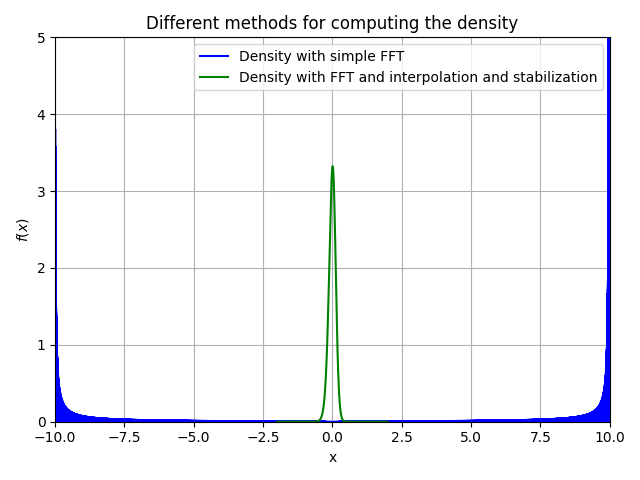
\includegraphics[width=0.8\textwidth]{img/different_ifft_methods.png}
    \caption{Comparison of different methods for the inverse Fourier transformation of the characteristic function of the Heston model ($\mu=0$, $\kappa=3$, $\theta=0.19$, $\sigma=0.4$, $\rho=-0.7$, $\tau=\frac{1}{12}$). Grid points: $N=2^{15}$.}
    \label{fig:ifft_comparison}
\end{figure}

\section{Simulating the Heston Model}

The Heston model is a continuous-time model, and for simulation purposes, time must be discretized. Small timesteps require significant computational power, while large timesteps may lead to zero or even negative volatility if the so-called Feller condition is not satisfied (\cite{albrecherLittleHestonTrap2007}). The Feller condition holds if $2\kappa\theta > \sigma^2$, but Eraker et al. (\citeyear{erakerImpactJumpsVolatility2003}) show that for S\&P 500 index options, this condition is violated. Many other studies confirm this result for various markets and asset classes (e.g., \cite{changOptionPricingDouble2021,huPricingVolatilityJump2022}).

The most intuitive approach to time discretization is the Euler–Maruyama scheme:
\begin{align}
    X_{t+\Delta} &= X_t - \frac{1}{2}v_t\Delta + \sqrt{v_t}\sqrt{\Delta}Z_{X,t} \notag \\
    v_{t+\Delta} &= v_t + \kappa(\theta - v_t)\Delta + \sigma\sqrt{v_t}\sqrt{\Delta}Z_{v,t} \notag
\end{align}
where $Z \sim \mathcal{N}(0,1)$, $\Delta = T/n$, with $T$ representing the total time and $n$ the number of time steps. The correlation between $Z_{X,t}$ and $Z_{v,t}$ can be simulated as follows (\cite{andersenEfficientSimulationHeston2007}): %TODO: andere Quelle finden, nicht immer nur Andersen oder Ostap
\begin{align}
    Z_{v,t} &= \Phi^{-1}(U_1) \notag \\
    Z_{X,t} &= \rho Z_{v,t} + \sqrt{1-\rho^2}\Phi^{-1}(U_2) \notag
\end{align}
where $U_1$ and $U_2$ are independent random variables uniformly distributed on $[0,1]$, and $\Phi^{-1}$ is the inverse cumulative distribution function of the standard normal distribution.

This discretization highlights the issue of potential negative volatility (\cite{okhrinSimulatingCoxIngersoll2022}):
\begin{align}
    \mathbb{P}(v_{t+\Delta}<0 \mid v_t>0) &= \mathbb{P}\left(Z_{v,t} < \frac{-v_t-\kappa(\theta-v_t)\Delta}{\sigma\sqrt{v_t}\sqrt{\Delta}}\right) \notag \\
    &= \Phi\left(Z_{v,t} < \frac{-v_t-\kappa(\theta-v_t)\Delta}{\sigma\sqrt{v_t}\sqrt{\Delta}}\right) \notag \\
    &> 0 \notag
\end{align}
where $\Phi$ denotes the cumulative distribution function of the standard normal distribution. Various methods exist to address this issue, such as the absorption method (replacing $v_t$ with $v_t^+ = \max(0, v_t)$) or the reflection method (replacing $v_t$ with $\vert v_t\vert$). However, these modifications alter the underlying process, causing the moments of volatility to deviate from their theoretical values (\cite{okhrinSimulatingCoxIngersoll2022,tsoskounoglouSimulatingHestonModel2024}).

In the study by Okhrin et al. (\citeyear{okhrinSimulatingCoxIngersoll2022}), Andersen's Quadratic Exponential (QE) scheme is found to perform best in terms of both speed and accuracy. Andersen (\citeyear{andersenEfficientSimulationHeston2007}) approximates the noncentral chi-square distribution in \eqref{eq:heston_model_variance_transition} using a mixture of distributions: a Dirac distribution and a noncentral Gaussian distribution. For sufficiently large values of $v_t$,
\begin{align}
    \label{eq:qe_normal}
    v_{t+\Delta} = a(b+Z_v)^2
\end{align}
where $Z_v \sim \mathcal{N}(0,1)$. For smaller values of $v_t$,
\begin{align}
    \label{eq:qe_dirac}
    v_{t+\Delta} &= \Psi^{-1}(U_v, p, \beta) \\
    \Psi^{-1}(u,p,\beta) &= \begin{cases}
        0 & 0\le u\le p \\
        \beta^{-1}\ln\left(\frac{1-p}{1-u}\right) & p<u\le 1
    \end{cases} \notag
\end{align}
The parameters $a$, $b$, $p$, and $\beta$ are estimated using moment matching and $U_v$ is drawn from a uniform distribution. The transition between the two approximation schemes is determined by a threshold $\psi_c$: if the ratio $\psi = s^2 / m^2$ (where $m$ and $s^2$ are the mean and variance of $v_{t+\Delta}$, respectively) exceeds $\psi_c$, then \eqref{eq:qe_dirac} is used; otherwise, \eqref{eq:qe_normal} is applied.

For the price process, Andersen (\citeyear{andersenEfficientSimulationHeston2007}) proposes the following discretization scheme:
\begin{align}
    \ln(S_{t+\Delta}) &= \ln(S_t) + K_0 + K_1v_t + K_2v_{t+\Delta} + \sqrt{K_3v_t + K_4v_{t+\Delta}}\cdot Z \notag \\
    K_0 &= -\frac{\rho\kappa\theta}{\sigma}\Delta \notag \\
    K_1 &= \xi_1\Delta\left(\frac{\kappa\rho}{\sigma} - \frac{1}{2}\right)-\frac{\rho}{\sigma} \notag \\
    K_2 &= \xi_2\Delta\left(\frac{\kappa\rho}{\sigma}-\frac{1}{2}\right)+\frac{\rho}{\sigma} \notag \\
    K_3 &= \xi_1\Delta(1-\rho^2) \notag \\
    K_4 &= \xi_2\Delta(1-\rho^2) \notag
\end{align}
where $Z$ is standard normally distributed, and $\xi_1$ and $\xi_2$ are constants. The paper suggests $\xi_1 = \xi_2 = 0.5$.

\section{The First 4 Moments of the Heston Model}

We now focus on the moments of the Heston Model but care must be taken with notation, as symbols such as $\mu$ and $\sigma$ usually denoting the mean and variance are now used to represent the drift and volatility of the Heston model (see Equations \eqref{eq:heston_model_price} and \eqref{eq:heston_model_variance}). The noncentral moments are denoted by $\mu_1$ through $\mu_4$, while the central and standardized moments are denoted by $\zeta_1$ through $\zeta_4$. It is possible to use the characteristic function to derive the moments of the Heston model:
\begin{align}
    \mu_k &= \mathrm{i}^{-k}\frac{\partial^k\phi(t)}{\partial t^k}\Bigg|_{t=0} \notag
\end{align}

Fortunately, moments for returns and other related measures have been derived. Okhrin et al. (\citeyear{okhrinSimulatingCoxIngersoll2022}) provide the unconditional noncentral moments for the log-return $r_t = \log(S_t) - \log(S_0)$:
\begin{align}
    \mu_1 &= \left(\mu - \frac{\theta}{2}\right)t \notag \\
    \mu_2 &= \frac{1}{4\kappa^3}\Biggl\{
        \exp(-\kappa t)\Biggl[
            \exp(\kappa t)\Bigl\{
                \kappa^3 t\Bigl[t(\theta-2\mu)^2 + 4\theta\Bigr] 
                - 4\kappa^2\rho\sigma t\theta \notag \\
            &\quad\quad + \kappa\sigma\theta(4\rho + \sigma t)
                - \sigma^2\theta
            \Bigr\} + \sigma\theta(\sigma-4\kappa\rho)
        \Biggr]
    \Biggr\} \notag
\end{align}
The expressions for $\mu_3$ and $\mu_4$ are too lengthy to be included here but can be found in Okhrin et al. (\citeyear{okhrinSimulatingCoxIngersoll2022}). The corresponding unconditional central and standardized moments are then given by:
\begin{align}
    \zeta_1 &= \mu_1 \notag \\
    \zeta_2 &= \mathbb{E}\left[(r_t-\mu_1)^2\right] \notag \\
    &=\frac{\theta}{4\kappa^3}\Biggl[
        -4\kappa^2\rho\sigma t + 4\kappa^3 t + \sigma\exp(-\kappa t)(\sigma - 4\kappa\rho) \notag\\
    &\quad\quad + 4\kappa\sigma\rho + \kappa\sigma^2 t - \sigma^2
    \Biggr] \notag \\
    \zeta_3 &= \mathbb{E}\left[\left(\frac{r_t-\mu_1}{\zeta_1^{1/2}}\right)^3\right] \notag \\
    &=\frac{3\kappa\sigma\theta\exp(\kappa t/2)(\sigma - 2\kappa\rho)}{\zeta_2^{3/2}}
    \Biggl[
        4\kappa^2\Bigl\{\exp(\kappa t)(\rho\sigma t+1) + \rho\sigma t - 1\Bigr\} \notag\\
    &\quad\quad - 4\kappa^3 t\exp(\kappa t) \notag\\
    &\quad\quad - \kappa\sigma\Bigl\{\exp(\kappa t)(8\rho + \sigma t) - 8\rho + \sigma t\Bigr\} \notag\\
    &\quad\quad + 2\sigma^2\Bigl(\exp(\kappa t)-1\Bigr)
    \Biggr] \notag \\
    \zeta_4 &= \mathbb{E}\left[\left(\frac{r_t-\mu_1}{\zeta_1^{1/2}}\right)^4\right] \notag
\end{align}
The expression for $\zeta_4$ is omitted here but can be found in Okhrin et al. (\citeyear{okhrinSimulatingCoxIngersoll2022}).

Zhao et al. (\citeyear{zhaoRelationPhysicalRiskneutral2013}) and Zhang et al.  (\citeyear{zhangSkewnessImpliedHeston2017}) analyze moments for the continuously compounded return $R_t^T = \ln\left(\frac{S_T}{S_t}\right)$ and derive the conditional central variance:
\begin{align}
    \mathbb{E}_t\Bigl(R_t^T-\mathbb{E}_t(R_t^T)\Bigr)^2 
    &= \frac{1}{4}\text{Var}_t\Biggl(\int_t ^T v_s\,\mathrm{d}s\Biggr) + SW_{t,T} \notag\\[1ex]
    &\quad - \mathbb{E}_t\Biggl(
        \int_t^T \sqrt{v_s}\,\mathrm{d}B_s
        \Biggl[\int_t^T v_s\,\mathrm{d}s-\mathbb{E}_t\Biggl(\int_t^T v_s\,\mathrm{d}s\Biggr)\Biggr]
    \Biggr) \notag
\end{align}    
where $v_t$ represents the variance at time $t$, $SW$ is the variance swap rate (the expectation of realized variance), and $B_t$ is a Brownian motion. Zhang et al. (\citeyear{zhangSkewnessImpliedHeston2017}) further elaborate:
\begin{align}
    \mathbb{E}_t\Bigl(R_t^T-\mathbb{E}_t(R_t^T)\Bigr)^2 &= \int_t^T \mathbb{E}_t(v_s)\,\mathrm{d}s \notag\\[1ex]
    &\quad - \rho\sigma\int_t^T \frac{1-\exp(-\kappa(T-s))}{\kappa}\mathbb{E}_t(v_s)\,\mathrm{d}s \notag\\[1ex]
    &\quad + \frac{1}{4}\Biggl(\sigma^2\int_t^T\frac{\Bigl(1-\exp(-\kappa(T-s))\Bigr)^2}{\kappa^2}\mathbb{E}_t(v_s) \,\mathrm{d}s\Biggr) \notag
\end{align}
    
Using the expected instantaneous variance $\mathbb{E}_t(v_s) = \theta + (v_t - \theta)\exp(-\kappa(s-t))$, Mathematica yields the following results:
\begin{align}
    \int_t^T \mathbb{E}_t(v_s)\,\mathrm{d}s 
    &= \frac{v_t - \theta + \exp\bigl(\kappa(t-T)\bigr)(-v_t+\theta) - t \theta\kappa + T\theta\kappa}{\kappa} \notag \\[1ex]
    \rho\sigma\int_t^T \frac{1-\exp\bigl(-\kappa(T-s)\bigr)}{\kappa}\mathbb{E}_t(v_s)\,\mathrm{d}s 
    &= \frac{\exp(-T\kappa)\,\rho\sigma}{\kappa^2} \Biggl[
        \exp(t\kappa)\Bigl(-v_t+2\theta+(t-T)
        \notag\\[1ex]
    &\quad\quad\times \Bigl[(v_t-\theta)\,\kappa\Bigr]\Bigr) \notag\\[1ex]
    &\quad\quad + \exp(T\kappa)\Bigl(v_t+\theta(-2-t\kappa+T\kappa)\Bigr)
    \Biggr] \notag \\[1ex]
    \sigma^2\int_t^T\frac{\bigl(1-\exp\bigl(-\kappa(T-s)\bigr)\bigr)^2}{\kappa^2}\mathbb{E}_t(v_s) \,\mathrm{d}s 
    &= \frac{\exp(-2T\kappa)\,\sigma^2}{2\kappa^3} \Biggl[
        \exp(2t\kappa)(-2v_t+\theta) \notag\\[1ex]
    &\quad\quad + 4\exp\bigl((t+T)\kappa\bigr)\Bigl(\theta+(t-T)(v_t-\theta)\kappa\Bigr) \notag\\[1ex]
    &\quad\quad + \exp(2T\kappa)\Bigl(2v_t+\theta(-5-2t\kappa+2T\kappa)\Bigr)
    \Biggr] \notag
\end{align}
The third conditional central moment is given by
\begin{align}
    \mathbb{E}_t(R_t^T-\mathbb{E}_t(R_t^T))^3 &= \mathbb{E}_t(X_T^3) - \frac{3}{2}\mathbb{E}_t(X_T^2Y_T) + \frac{3}{4}\mathbb{E}_t(X_TY_T^2) - \frac{1}{8}\mathbb{E}_t(Y_T^3) \notag
\end{align}
where $X_T$ and $Y_T$ are defined as
\begin{align}
    X_T &= \int_t^T \sqrt{v_s}\,\mathrm{d}B_s^S \notag \\
    Y_T &= \int_t^T (v_s - \mathbb{E}_t(v_s))\,\mathrm{d}s = \sigma\int_t^T\frac{1-\exp(-\kappa(T-s))}{\kappa}\sqrt{v_s}\,\mathrm{d}B_s^v \notag
\end{align}
where $B^S$ and $B^v$ are the Brownian motions associated with price and volatility, respectively.

Dunn et al. (\citeyear{dunnEstimatingOptionPrices2014}) derive the unconditional noncentral moments for the return $Q_{t+1}=\frac{S_{t+1}}{S_t}$:
\begin{align}
    \mathbb{E}(Q_{t+1}) &= \mu_1 = 1+\mu  \notag \\
    \mathbb{E}(Q_{t+1}^2) &= \mu_2 = (\mu+1)^2+\theta \notag \\
    \mathbb{E}(Q_{t+1}^3) &= \mu_3 = (\mu+1)^3+3\theta+3\mu\theta \notag \\
    \mathbb{E}(Q_{t+1}^4) &= \mu_4 \notag \\
    &=\frac{1}{\kappa(\kappa-2)}\Biggl(
        \kappa^2\mu^4 + 4\kappa^2\mu^3 + 6\kappa^2\mu^2\theta - 2\kappa\mu^4 \notag\\[1ex]
    &\quad\quad +\, 6\kappa^2\mu^2 + 12\kappa^2\mu\theta + 3\kappa^2\theta^2 - 8\kappa\mu^3 \notag\\[1ex]
    &\quad\quad -\, 12\kappa\mu^2\theta + 4\kappa^2\mu + 6\kappa^2\theta - 12\kappa\mu^2 \notag\\[1ex]
    &\quad\quad -\, 24\kappa\mu\theta - 6\kappa\theta^2 - 3\sigma^2\theta + \kappa^2 \notag\\[1ex]
    &\quad\quad -\, 8\kappa\mu - 12\kappa\theta - 2\kappa
    \Biggr) \notag
\end{align}
Using Equations \eqref{eq:definition_variance}, \eqref{eq:definition_skewness}, and \eqref{eq:definition_kurtosis}, the central and standardized moments follow as
\begin{align}
    \zeta_1 &= 1+\mu \notag \\
    \zeta_2 &= \theta \notag \\
    \zeta_3 &= 0 \notag \\
    \zeta_4 &= 3\frac{\kappa^2\theta - 2\kappa\theta - \sigma^2}{\kappa\theta(\kappa-2)} \notag
\end{align}